\section{Frequency mode 01}
\label{sec:fm01}

\subsection{Overview}
\label{sec:fm01:overview}
Frequency mode~01 monitors two bands, $501.180$--$501.580\,\mathrm{GHz}$ and
$501.980$--$502.380\,\mathrm{GHz}$. Its main use is retrievals of \chem{O_3},
\chem{ClO} and \chem{N_2O}.
\TODO{General text about FM01}
\TODO{Show spectra?}

\subsection{Comparison of retrieved profiles}
\label{sec:fm01:comparison}
\TODO{Averaging kernels}


%%%%%%
% O3 %
%%%%%%

\subsubsection{\chem{O_3}}
\label{sec:fm01:comparison:O3}
The retrievals for \chem{O_3} have been compared with data from the MIPAS, MLS,
OSIRIS and SAGE~III instruments. Annual average differences to these
instruments are shown in Figure~\ref{fig:fm01:O3:profiles}. In
Figure~\ref{fig:fm01:O3:scatter} individual retrievals for the instruments for
the entire period are plotted against the retrievals from the new and old
versions of the \smr\ processing chain. The results show a considerable
improvement with the updated version of the processing, with much better
over-all correlation and most of the systematic under estimation having been
removed compared to all instruments except for SAGE~III. Compared to SAGE~III,
the results were bad for \smr~v2.X, but are even worse for \smr~v3. This may be
attributed to the fact that the collocated measurments for SAGE~III are all
from altitude range $40$--$50$~km, which is the upper range of altitudes for
this frequency mode, and the lower range for the SAGE~III instrument, as seen
in Figure~\ref{fig:fm01:O3:profiles:SAGEIII}.
\TODO{reference Fig.~\ref{fig:fm01:O3:mr_avk} in text!}

\begin{figure}[htpb]
    \centering
    \begin{subfigure}[b]{0.49\textwidth}
        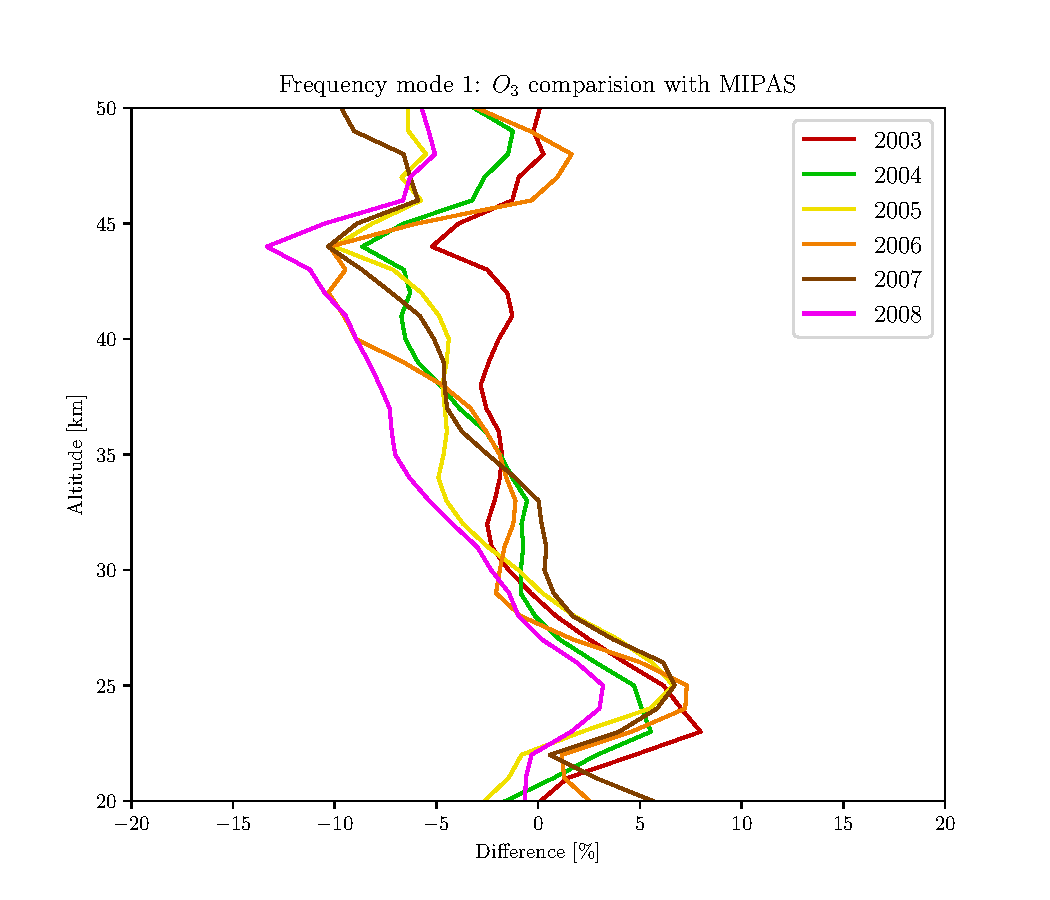
\includegraphics[width=\textwidth]{DDS_fm1_O3_perdiff_mipas}
        \caption{average difference to MIPAS}
        \label{fig:fm01:O3:profiles:MIPAS}
    \end{subfigure}
    \,
    \begin{subfigure}[b]{0.49\textwidth}
        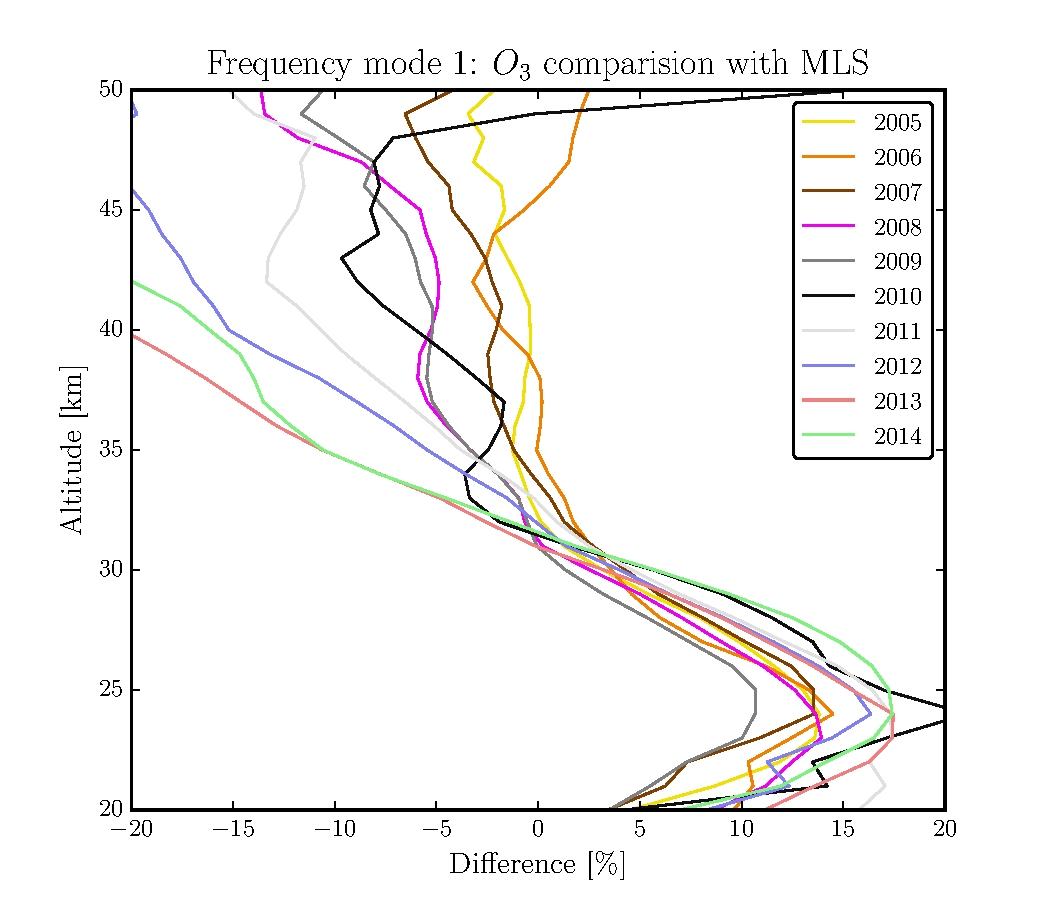
\includegraphics[width=\textwidth]{DDS_fm1_O3_perdiff_mls}
        \caption{average difference to MLS}
        \label{fig:fm01:O3:profiles:MLS}
    \end{subfigure}

    \begin{subfigure}[b]{0.49\textwidth}
        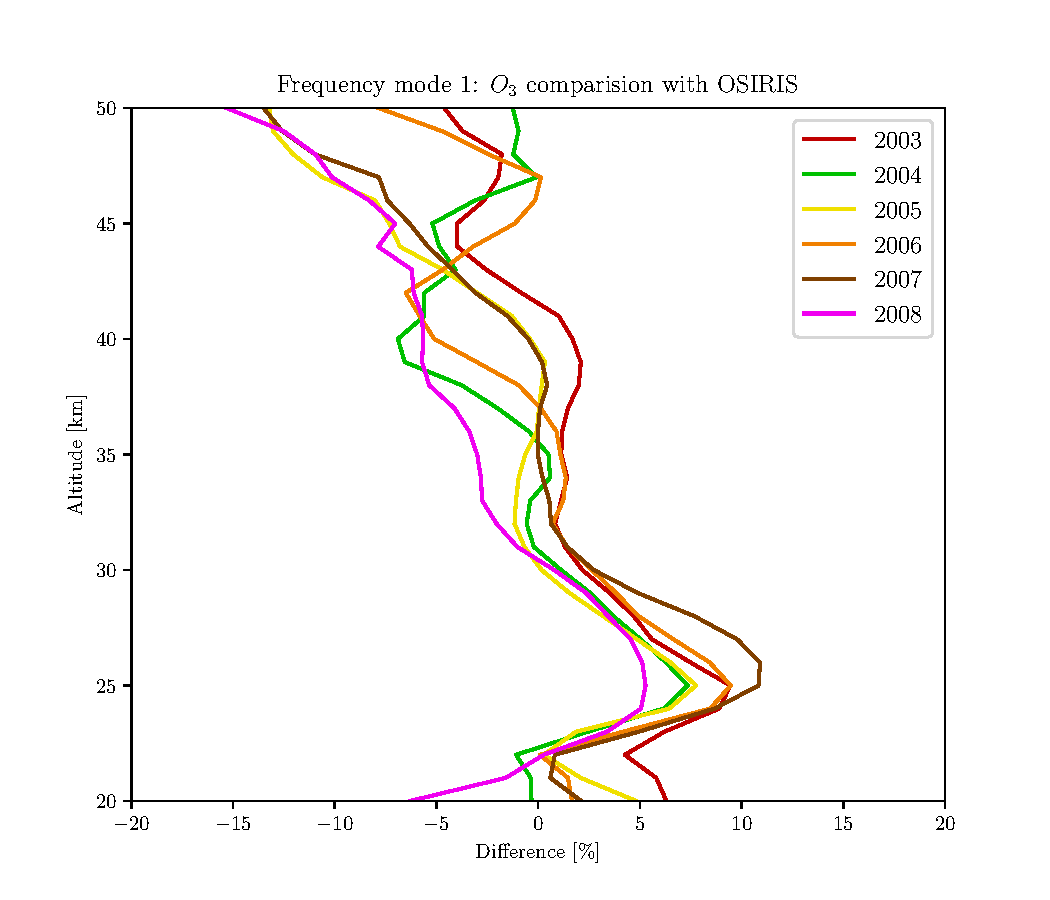
\includegraphics[width=\textwidth]{DDS_fm1_O3_perdiff_osiris}
        \caption{average difference to OSIRIS}
        \label{fig:fm01:O3:profiles:OSIRIS}
    \end{subfigure}
    \,
    \begin{subfigure}[b]{0.49\textwidth}
        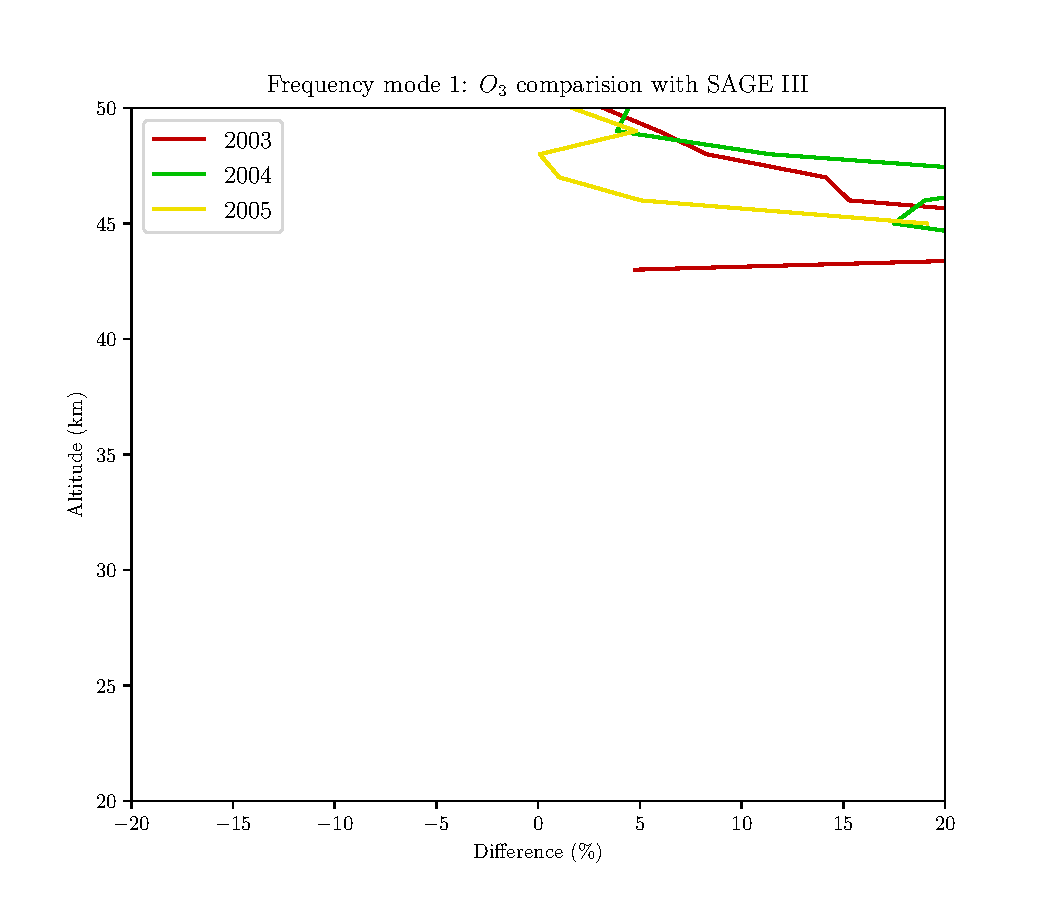
\includegraphics[width=\textwidth]{DDS_fm1_O3_perdiff_sage}
        \caption{average difference to SAGEIII}
        \label{fig:fm01:O3:profiles:SAGEIII}
    \end{subfigure}
    \caption{Average difference in percent between retrievals of \chem{O_3}
    from \smr~v3 and collocated measurements from various instruments at
    different altitudes for frequency mode~01.}
    \label{fig:fm01:O3:profiles}
\end{figure}

\begin{figure}[htpb]
    \centering
    \begin{subfigure}[b]{0.49\textwidth}
        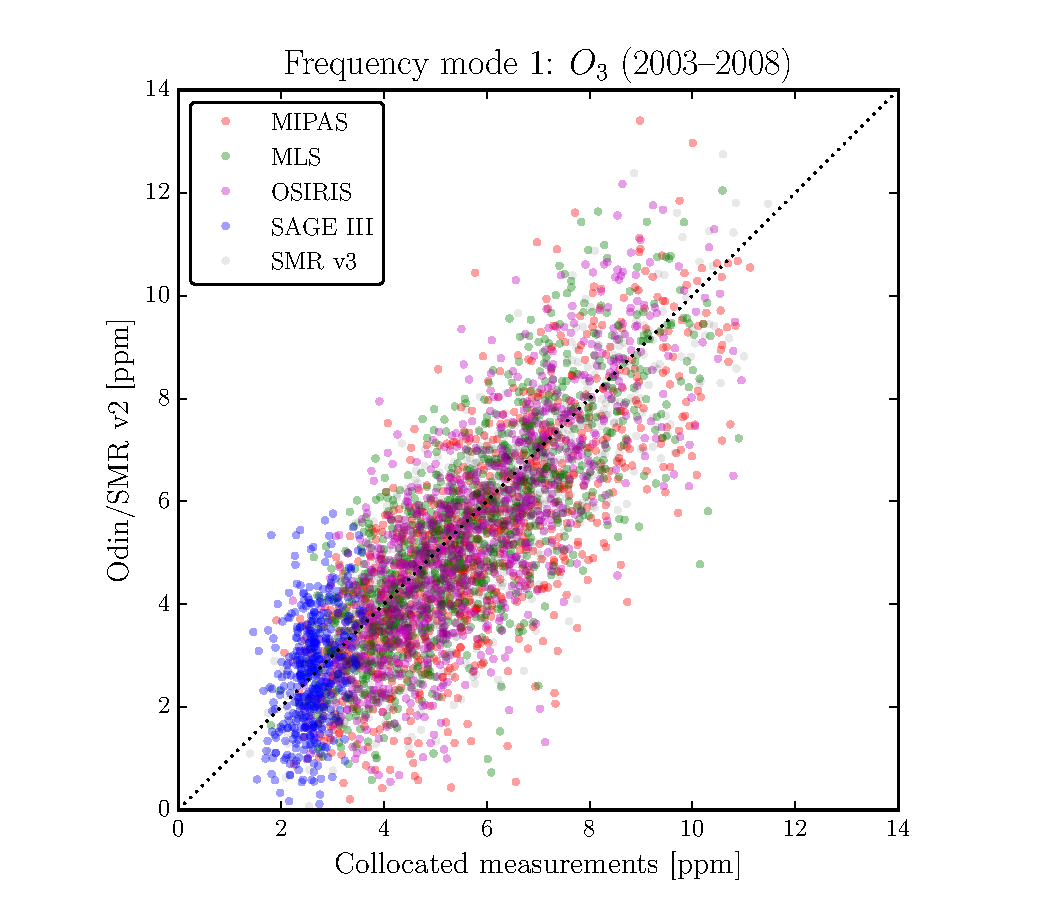
\includegraphics[width=\textwidth]{DDS_fm1_O3_scatter_v2}
        \caption{correlation of collcated instruments with \smr~v2.X}
        \label{fig:fm01:O3:scatter:v2}
    \end{subfigure}
    \,
    \begin{subfigure}[b]{0.49\textwidth}
        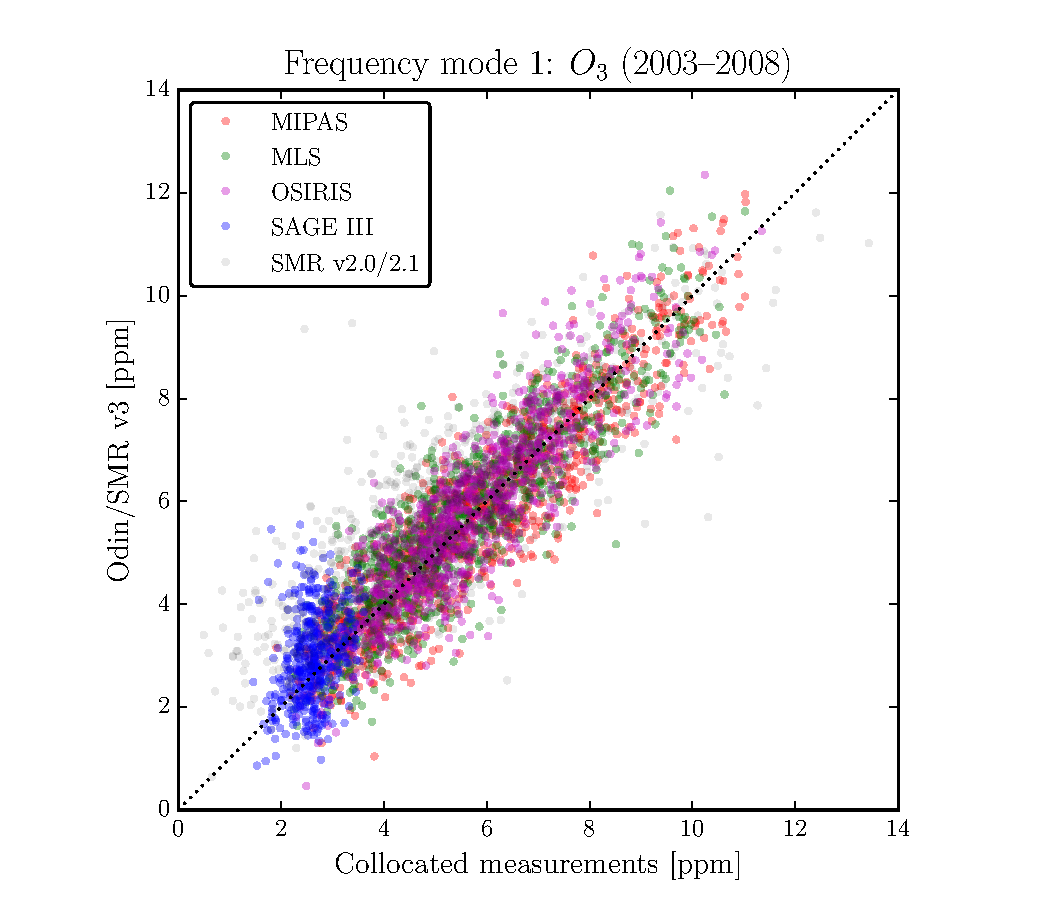
\includegraphics[width=\textwidth]{DDS_fm1_O3_scatter_v3}
        \caption{correlation of collcated instruments with \smr~v3}
        \label{fig:fm01:O3:scatter:v3}
    \end{subfigure}
    \caption{Correlation between retrievals of \chem{O_3} using \smr\
    versions~2.X and~3 and collocated measurements from various instruments
    for frequency mode~01.}
    \label{fig:fm01:O3:scatter}
\end{figure}

\begin{figure}[htpb]
    \centering
    \begin{subfigure}[b]{0.49\textwidth}
        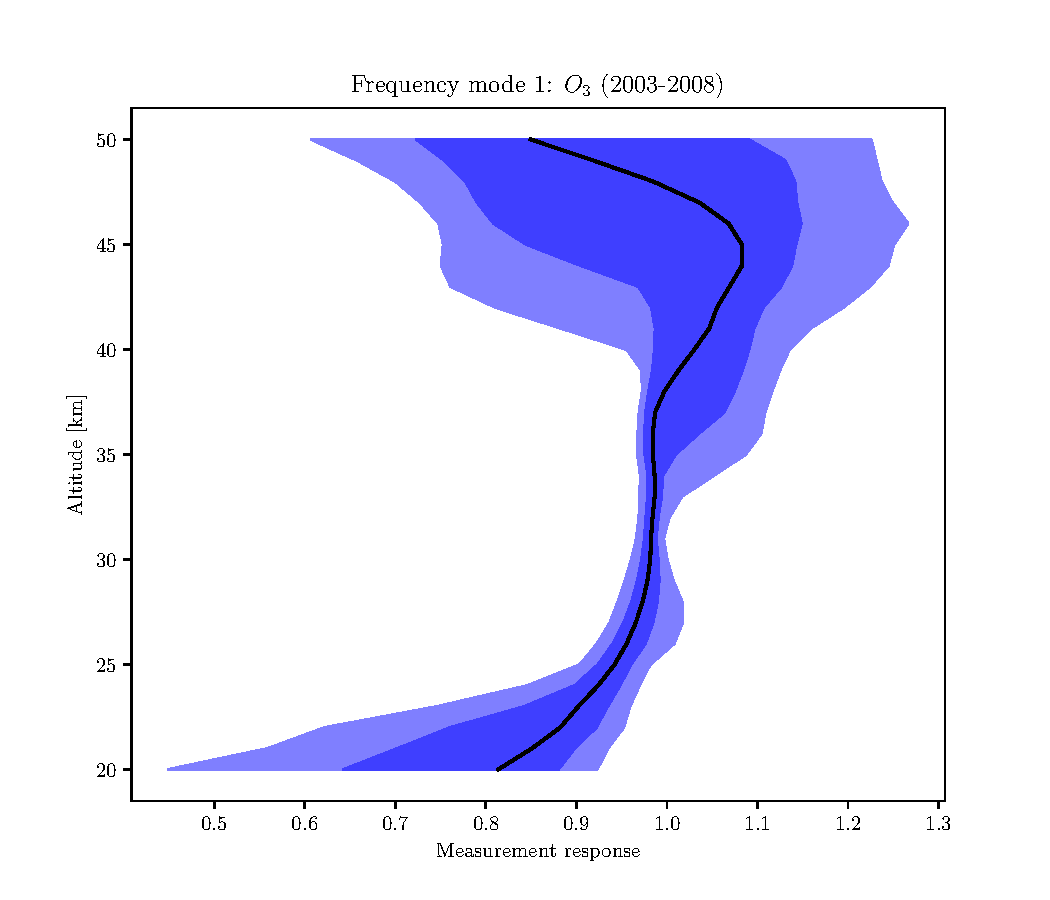
\includegraphics[width=\textwidth]{DDS_fm1_O3_mr}
        \caption{median measurement response with $1\sigma$ and $2\sigma$
        percentiles}
        \label{fig:fm01:O3:mr}
    \end{subfigure}
    \,
    \begin{subfigure}[b]{0.49\textwidth}
        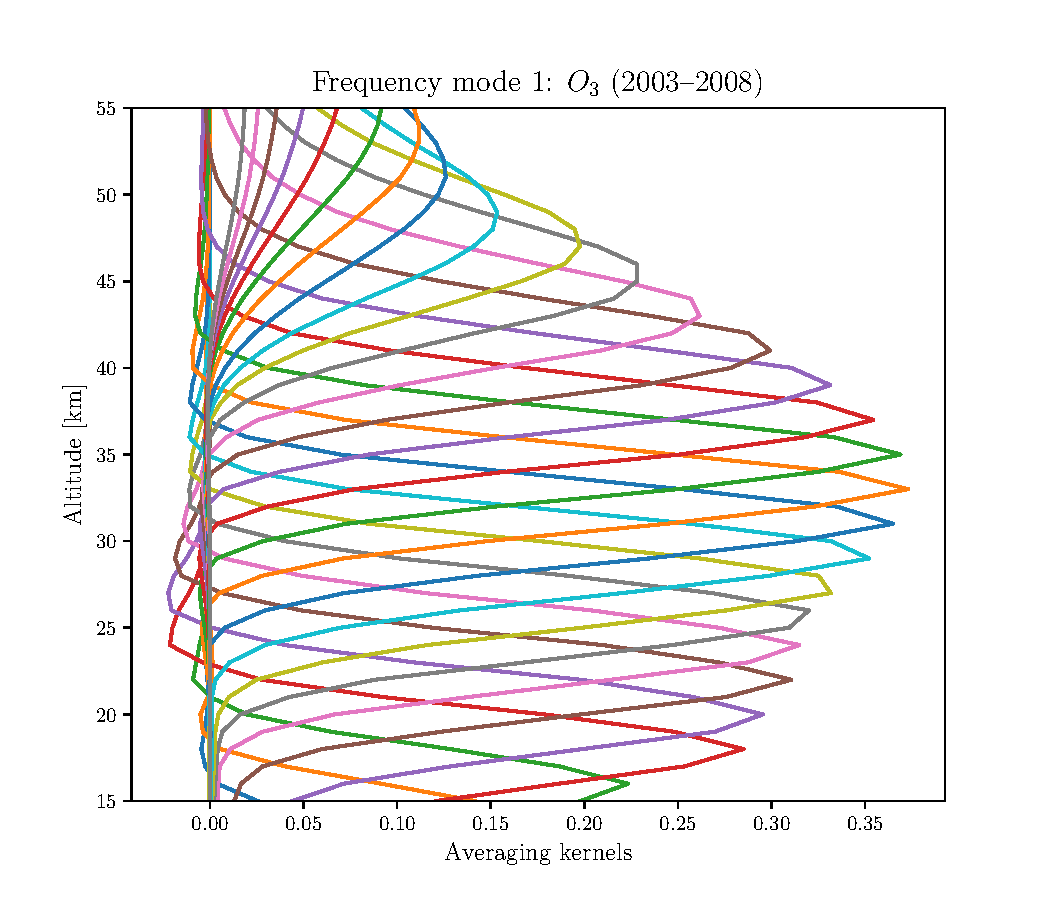
\includegraphics[width=\textwidth]{DDS_fm1_O3_avk}
        \caption{median averaging kernels\newline~}
        \label{fig:fm01:O3:avk}
    \end{subfigure}
    \caption{Measurement response and averaging kernels for \chem{O_3}
    retrievals for \smr~v3 at different altitudes for frequency mode~01.}
    \label{fig:fm01:O3:mr_avk}
\end{figure}


%%%%%%%
% N2O %
%%%%%%%

\subsubsection{\chem{N_2O}}
\label{sec:fm01:comparison:N2O}
The retrievals for \chem{N_2O} have been compared with data from the MIPAS and
MLS instruments. Annual average differences to these instruments are shown in
Figure~\ref{fig:fm01:N2O:profiles}. In Figure~\ref{fig:fm01:N2O:scatter}
individual retrievals for the instruments for the entire period are plotted
against the retrievals from the new and old versions of the \smr\ processing
chain. Only a minor improvement is seen with the updated version of the
processing.
\TODO{reference Fig.~\ref{fig:fm01:N2O:mr_avk} in text!}

\begin{figure}[htpb]
    \centering
    \begin{subfigure}[b]{0.49\textwidth}
        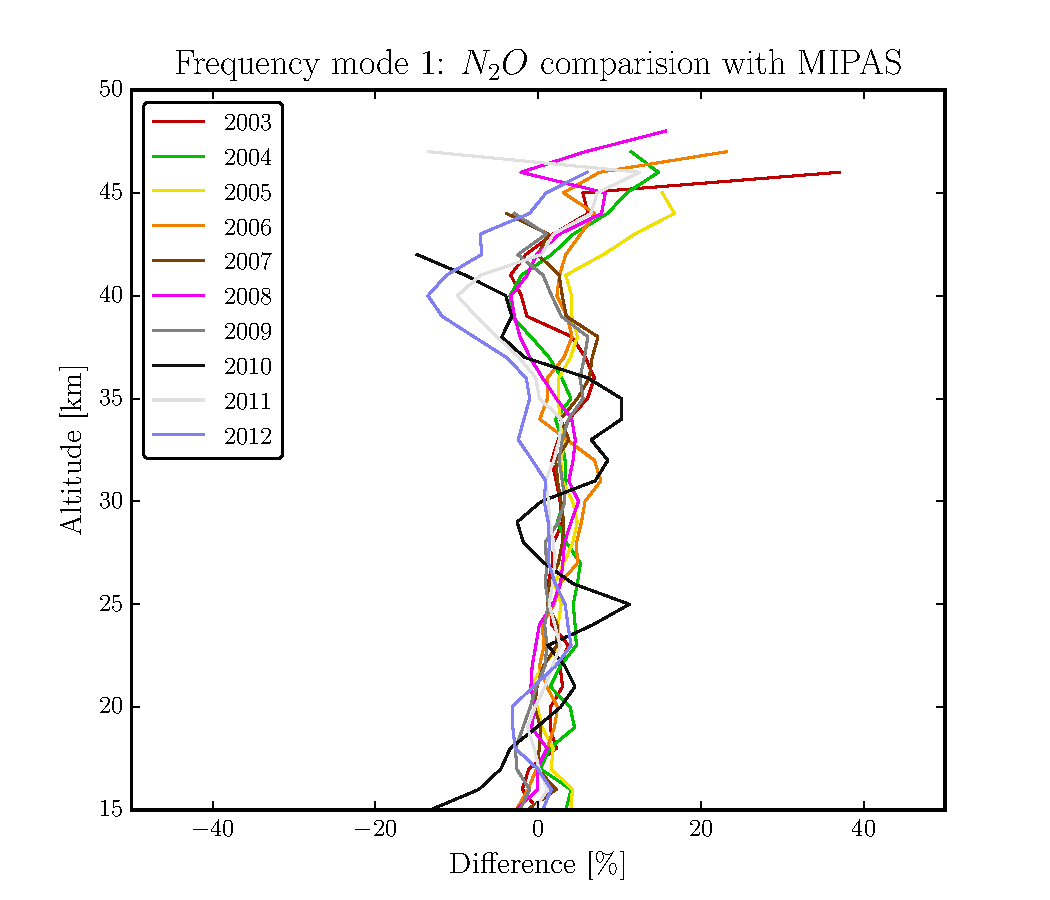
\includegraphics[width=\textwidth]{DDS_fm1_N2O_perdiff_mipas}
        \caption{average difference to MIPAS}
        \label{fig:fm01:N2O:profiles:MIPAS}
    \end{subfigure}
    \,
    \begin{subfigure}[b]{0.49\textwidth}
        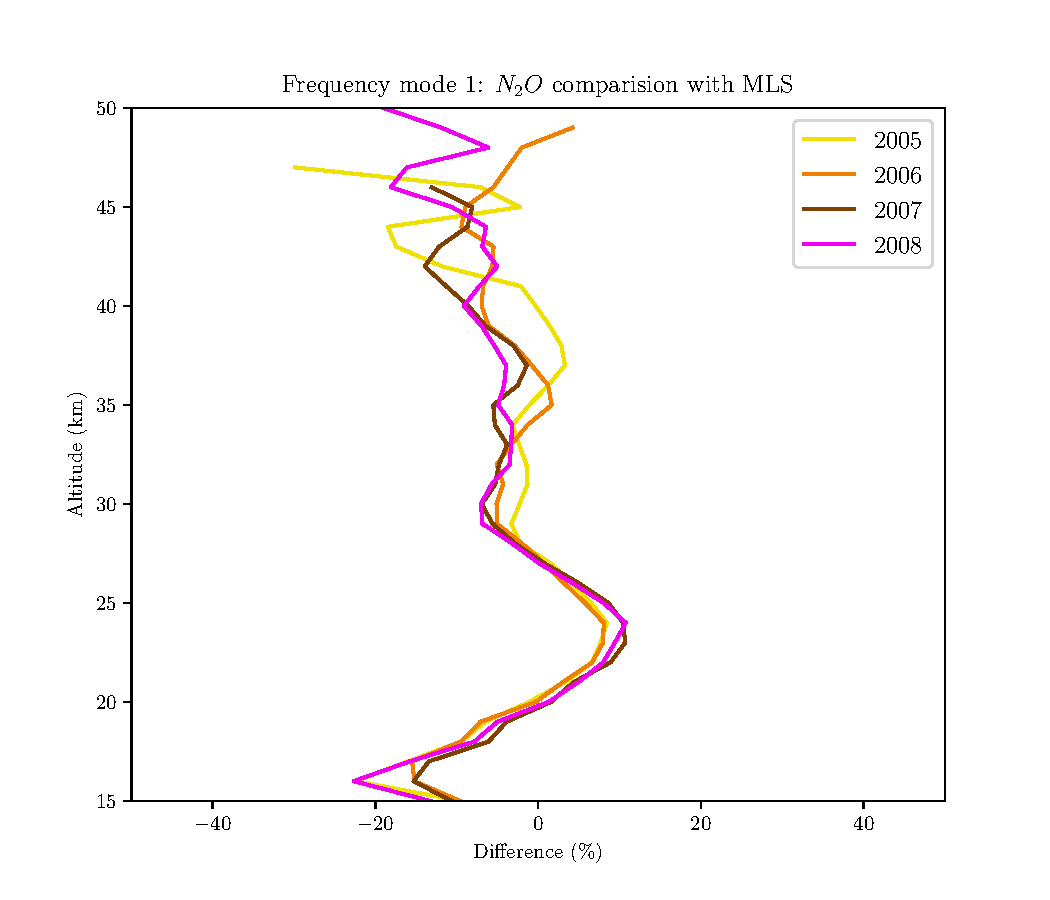
\includegraphics[width=\textwidth]{DDS_fm1_N2O_perdiff_mls}
        \caption{average difference to MLS}
        \label{fig:fm01:N2O:profiles:MLS}
    \end{subfigure}
    \caption{Average difference in percent between retrievals of \chem{N_2O}
    from \smr~v3 and collocated measurements from various instruments at
    different altitudes for frequency mode~01. (Retrievals yielding
    concentrations $\leq 0.03\,\mathrm{ppm}$ have been filtered out.)}
    \label{fig:fm01:N2O:profiles}
\end{figure}

\begin{figure}[htpb]
    \centering
    \begin{subfigure}[b]{0.49\textwidth}
        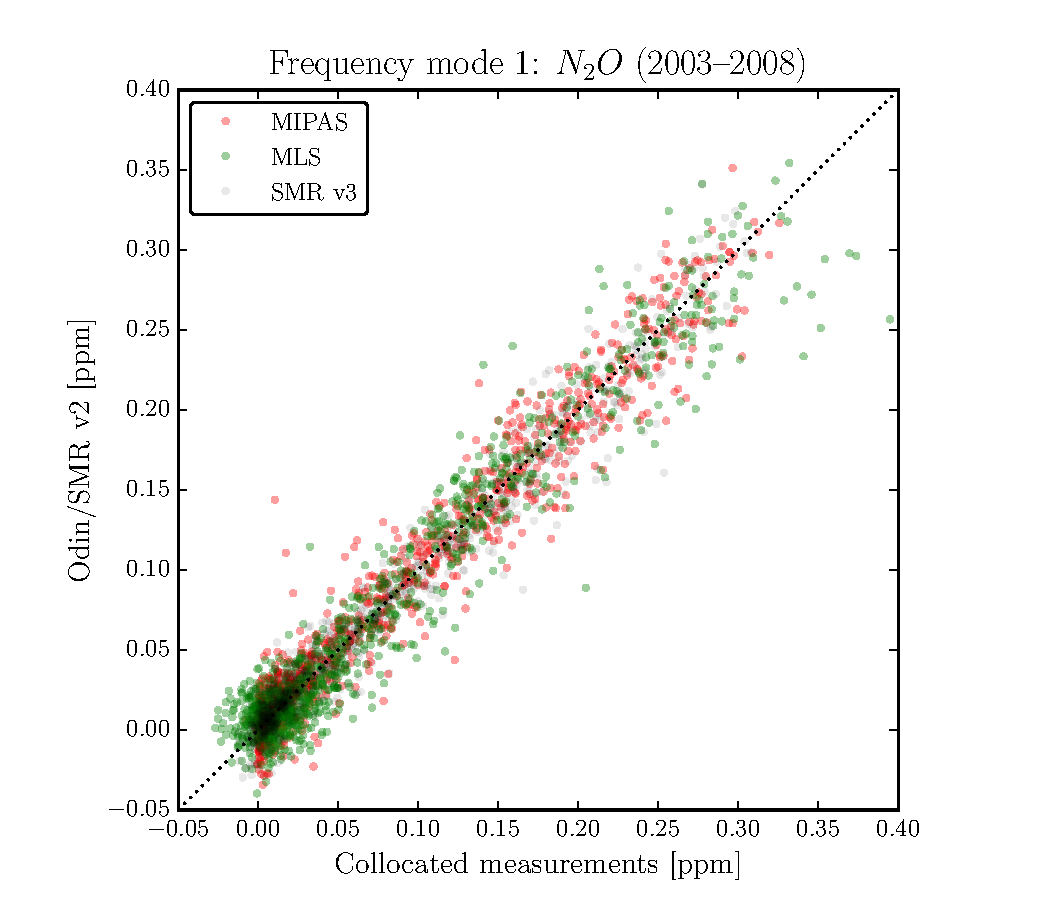
\includegraphics[width=\textwidth]{DDS_fm1_N2O_scatter_v2}
        \caption{correlation of collcated instruments with \smr~v2.X}
        \label{fig:fm01:N2O:scatter:v2}
    \end{subfigure}
    \,
    \begin{subfigure}[b]{0.49\textwidth}
        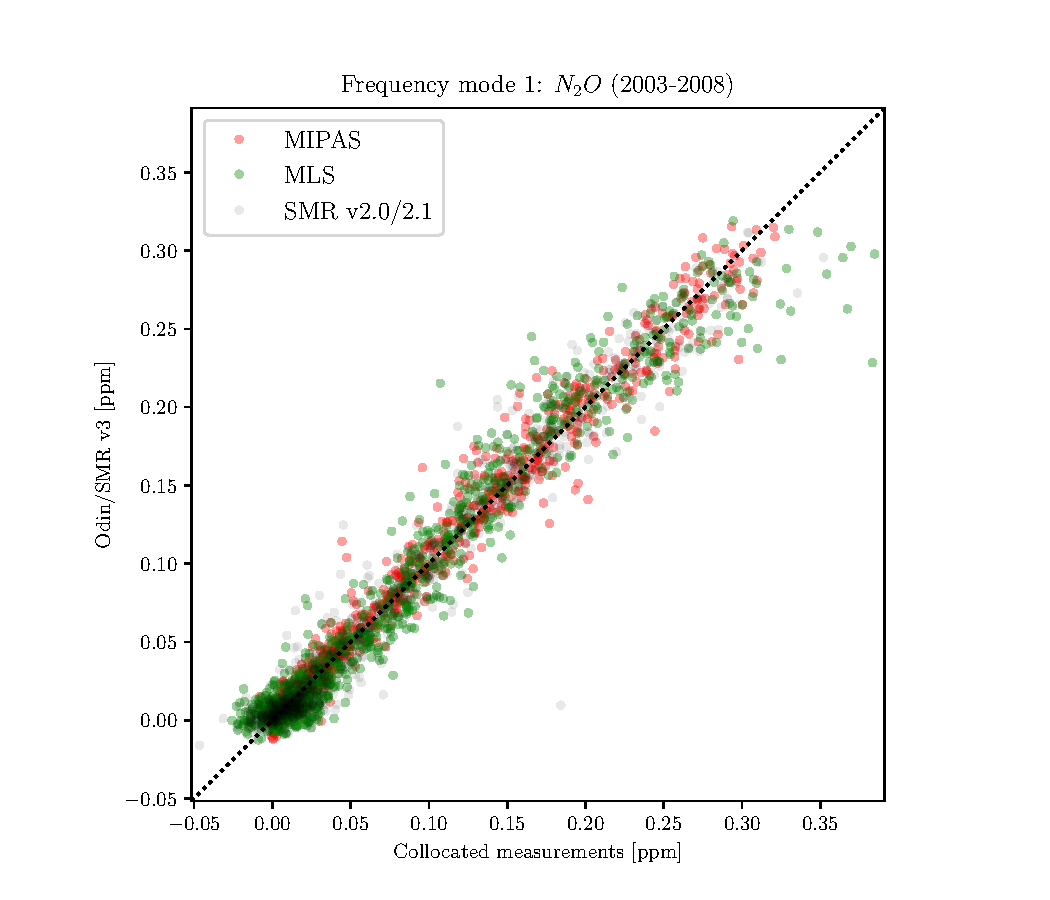
\includegraphics[width=\textwidth]{DDS_fm1_N2O_scatter_v3}
        \caption{correlation of collcated instruments with \smr~v3}
        \label{fig:fm01:N2O:scatter:v3}
    \end{subfigure}
    \caption{Correlation between retrievals of \chem{N_2O} using \smr\
    versions~2.X and~3 and collocated measurements from various instruments
    for frequency mode~01.}
    \label{fig:fm01:N2O:scatter}
\end{figure}

\begin{figure}[htpb]
    \centering
    \begin{subfigure}[b]{0.49\textwidth}
        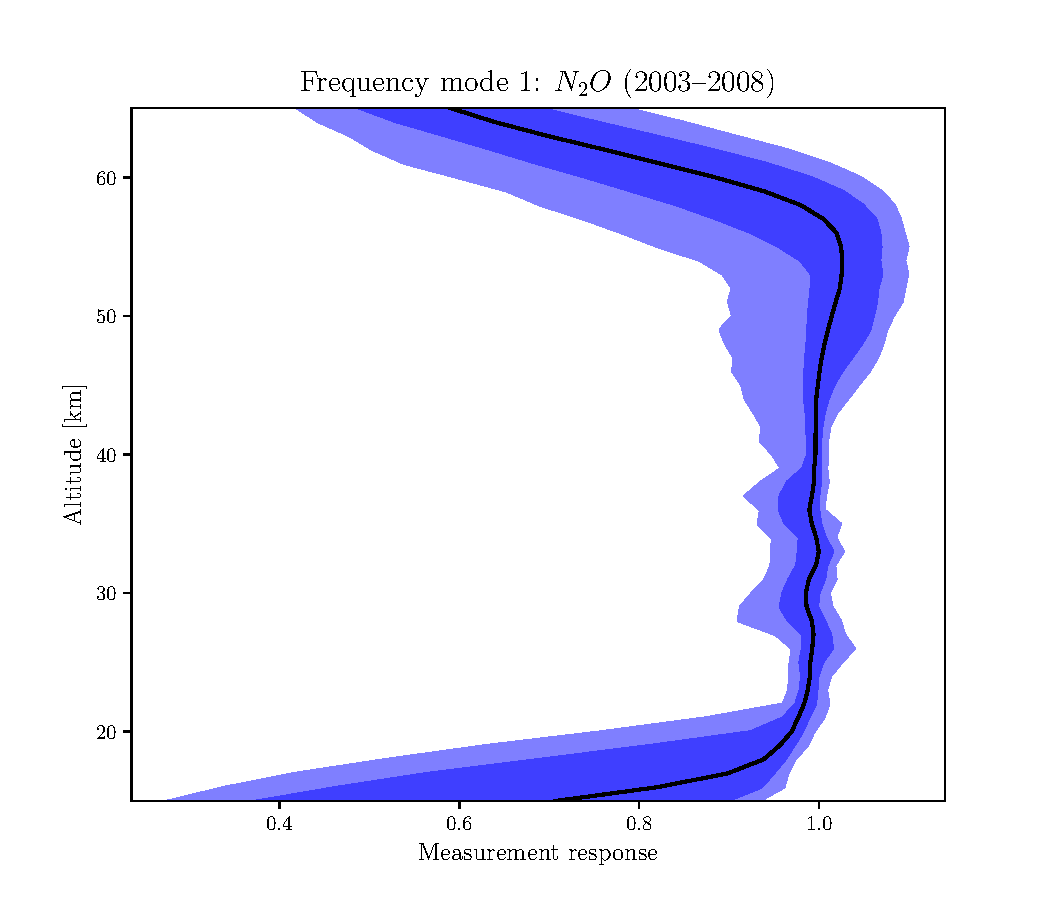
\includegraphics[width=\textwidth]{DDS_fm1_N2O_mr}
        \caption{median measurement response with $1\sigma$ and $2\sigma$
        percentiles}
        \label{fig:fm01:N2O:mr}
    \end{subfigure}
    \,
    \begin{subfigure}[b]{0.49\textwidth}
        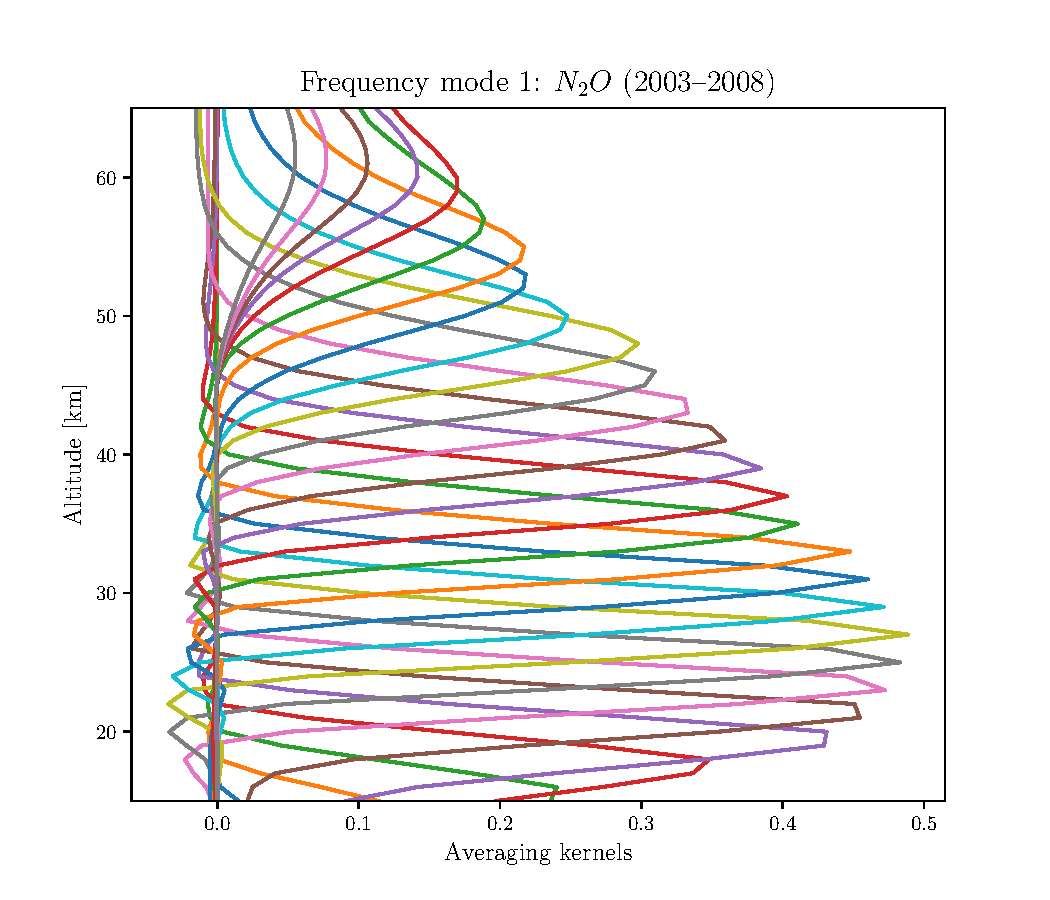
\includegraphics[width=\textwidth]{DDS_fm1_N2O_avk}
        \caption{median averaging kernels\newline~}
        \label{fig:fm01:N2O:avk}
    \end{subfigure}
    \caption{Measurement response and averaging kernels for \chem{N_2O}
    retrievals for \smr~v3 at different altitudes for frequency mode~01.}
    \label{fig:fm01:N2O:mr_avk}
\end{figure}


%%%%%%%
% ClO %
%%%%%%%

\subsubsection{\chem{ClO}}
\label{sec:fm01:comparison:ClO}
The retrievals for \chem{ClO} have been compared with data from the MLS
instrument. Annual average differences to MLS are shown in
Figure~\ref{fig:fm01:ClO:profiles}. In Figure~\ref{fig:fm01:ClO:scatter}
individual retrievals from MLS for the entire period are plotted against the
retrievals from the new and old versions of the \smr\ processing chain. No
sizeable improvement is seen for the new version of the \smr\ processing chain
compared to MLS, and the correlation between the two remains poor, however,
Figure~\ref{fig:fm01:ClO:scatter} suggests that this is due to noisy nature of
the MLS retrievals, which show a very large spread -- sometimes even large
negative concentrations -- for the retrievals where both \smr\ versions yield
low \chem{ClO} concentrations. An alternative explanation is that, since
\chem{ClO} concentrations have a diurnal cycle, collocation in time is very
important for comparisons, and due to the orbits of the two instruments, this
is only really satisfied near the poles.
\TODO{reference Fig.~\ref{fig:fm01:ClO:mr_avk} in text!}

\begin{figure}[htpb]
    \centering
    \begin{subfigure}[b]{0.49\textwidth}
        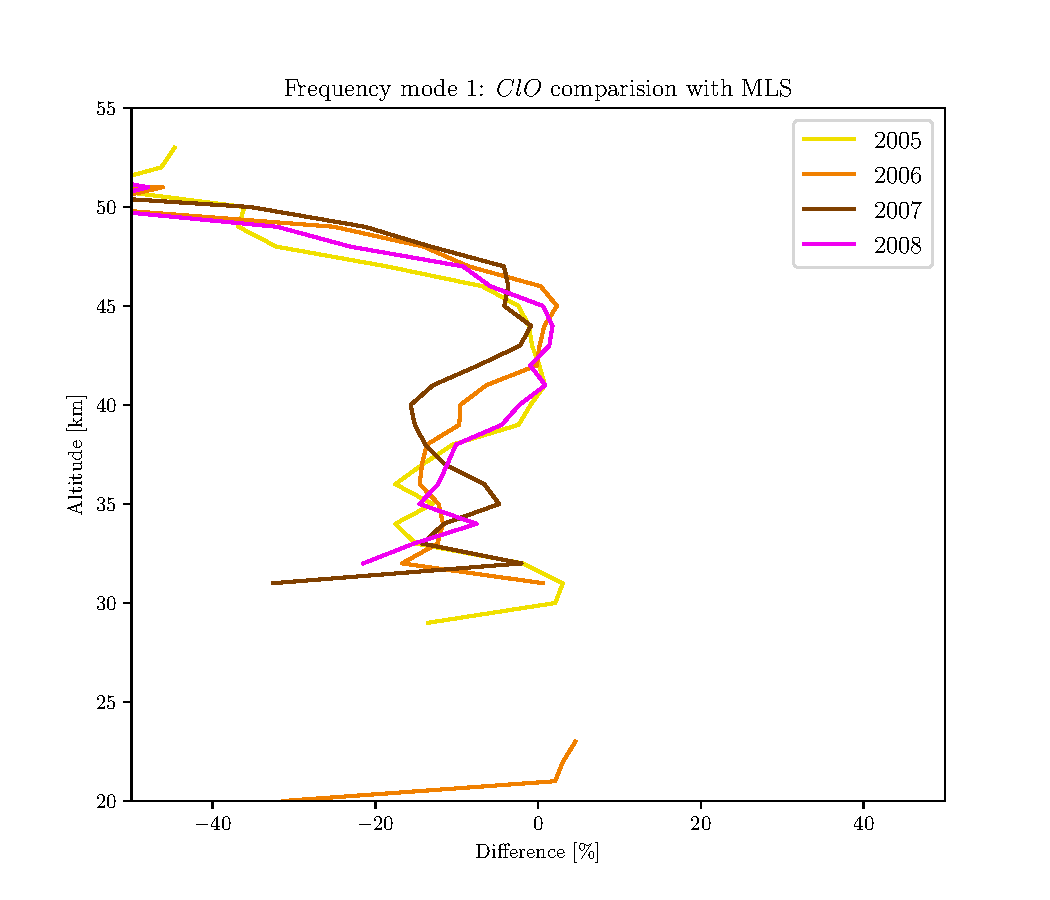
\includegraphics[width=\textwidth]{DDS_fm1_ClO_perdiff_mls}
        \caption{average difference to MLS}
        \label{fig:fm01:ClO:profiles:MLS}
    \end{subfigure}
    \caption{Average difference in percent between retrievals of \chem{N_2O}
    from \smr~v3 and collocated measurements from various instruments at
    different altitudes for frequency mode~01. (Retrievals yielding
    concentrations $\leq 0.3\,\mathrm{ppb}$ have been filtered out.)}
    \label{fig:fm01:ClO:profiles}
\end{figure}

\begin{figure}[htpb]
    \centering
    \begin{subfigure}[b]{0.49\textwidth}
        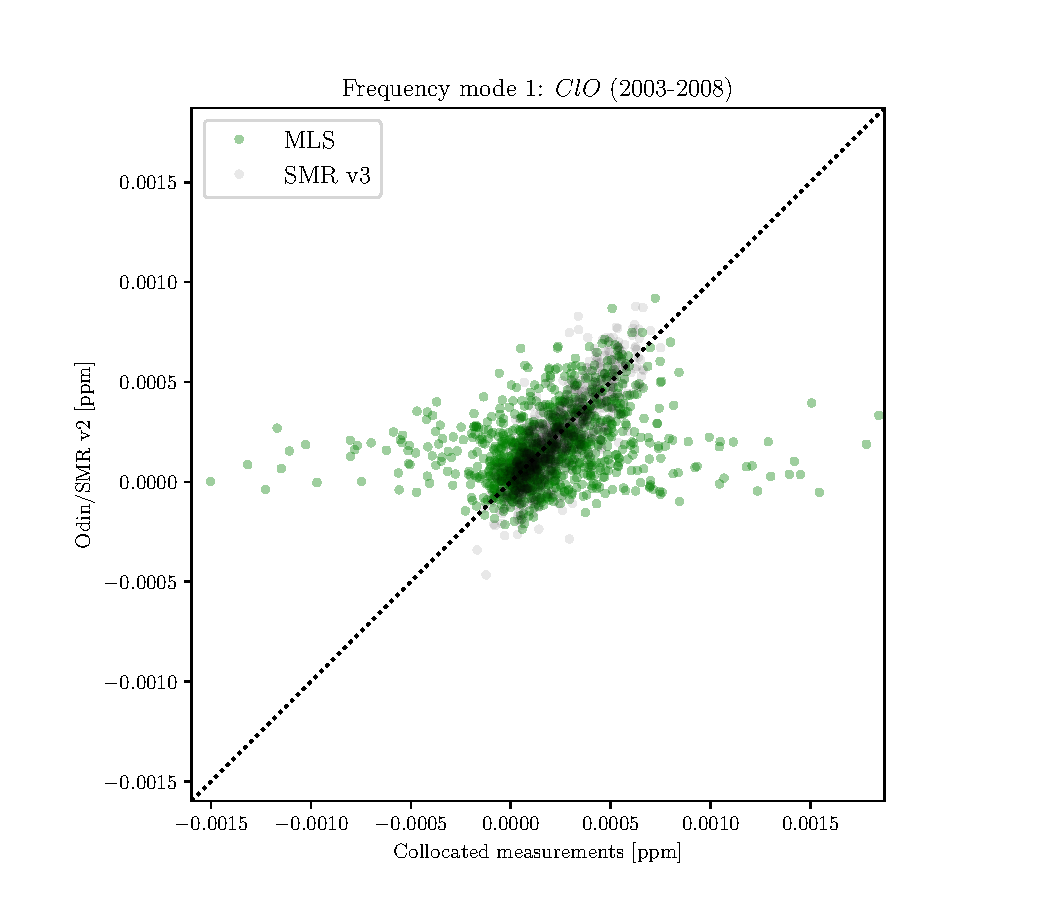
\includegraphics[width=\textwidth]{DDS_fm1_ClO_scatter_v2}
        \caption{correlation of collcated MLS measurements with \smr~v2.X}
        \label{fig:fm01:ClO:scatter:v2}
    \end{subfigure}
    \,
    \begin{subfigure}[b]{0.49\textwidth}
        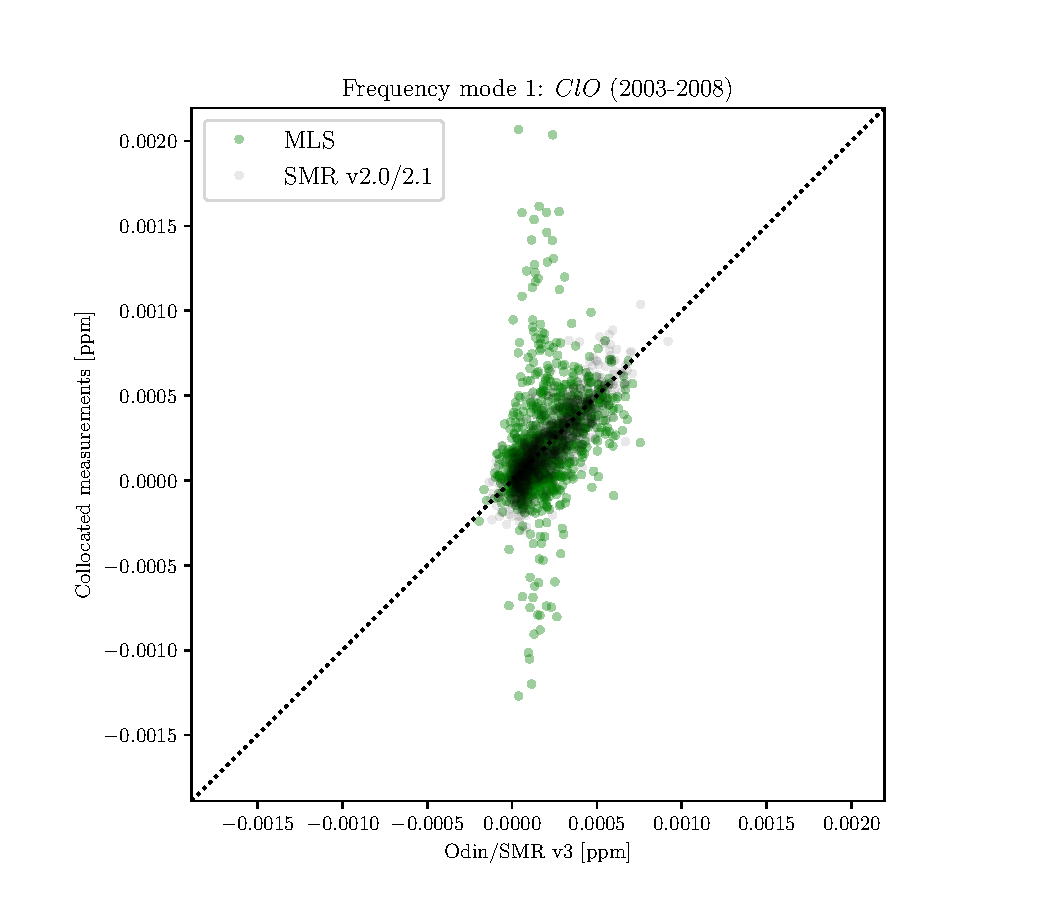
\includegraphics[width=\textwidth]{DDS_fm1_ClO_scatter_v3}
        \caption{correlation of collcated MLS measurements with \smr~v3}
        \label{fig:fm01:ClO:scatter:v3}
    \end{subfigure}
    \caption{Correlation between retrievals of \chem{N_2O} using \smr\
    versions~2.X and~3 and collocated measurements MLS for frequency mode~01.}
    \label{fig:fm01:ClO:scatter}
\end{figure}

\begin{figure}[htpb]
    \centering
    \begin{subfigure}[b]{0.49\textwidth}
        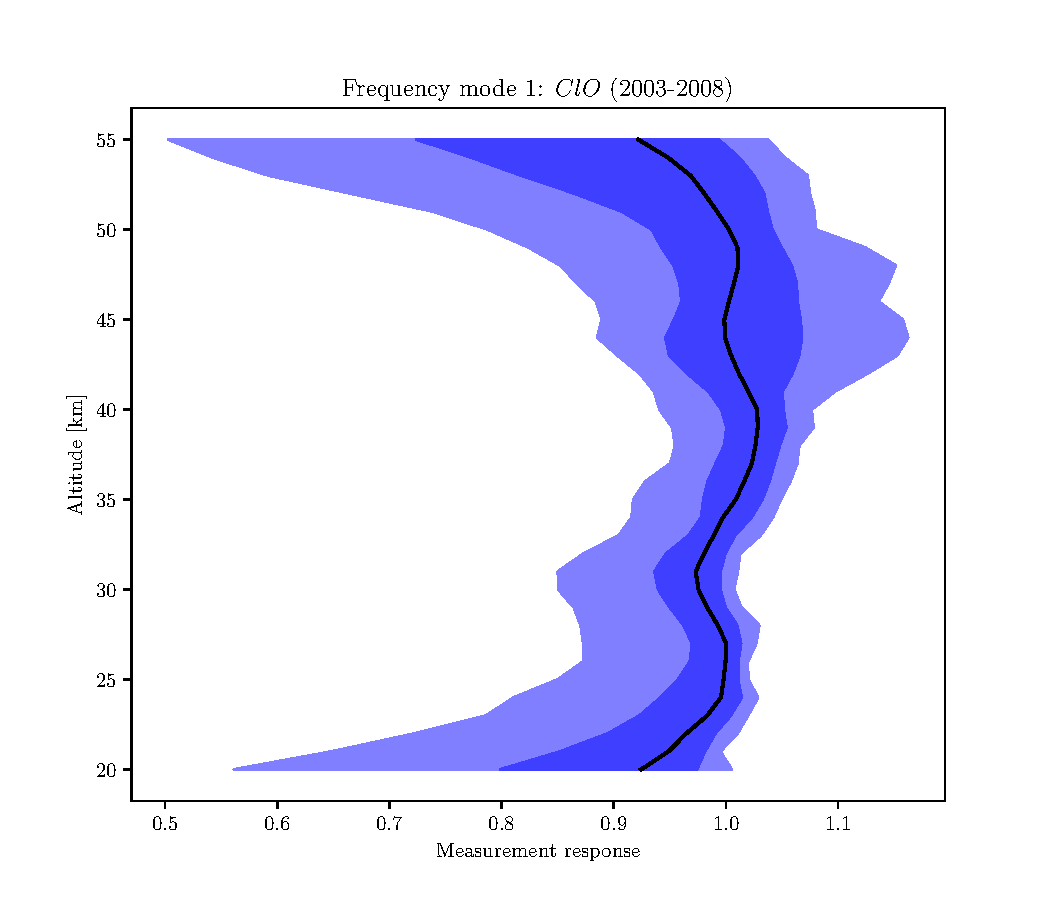
\includegraphics[width=\textwidth]{DDS_fm1_ClO_mr}
        \caption{median measurement response with $1\sigma$ and $2\sigma$
        percentiles}
        \label{fig:fm01:ClO:mr}
    \end{subfigure}
    \,
    \begin{subfigure}[b]{0.49\textwidth}
        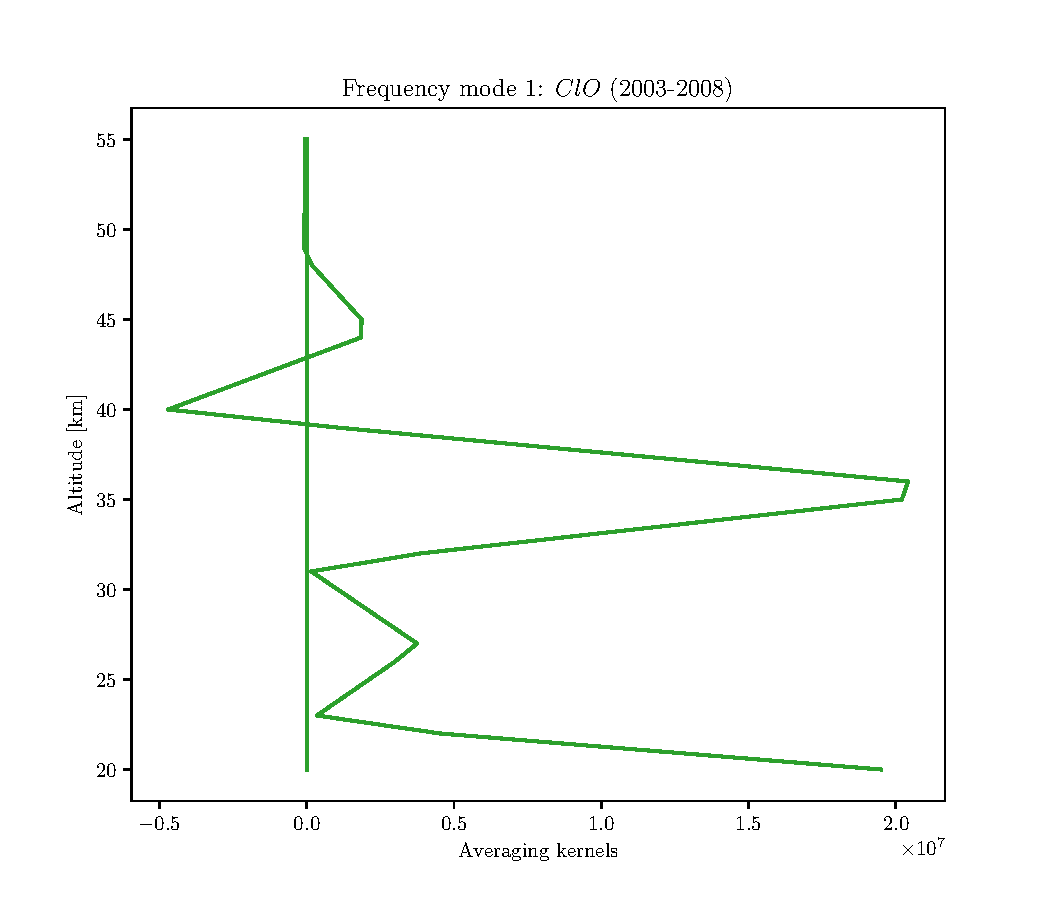
\includegraphics[width=\textwidth]{DDS_fm1_ClO_avk}
        \caption{median averaging kernels\newline~}
        \label{fig:fm01:ClO:avk}
    \end{subfigure}
    \caption{Measurement response and averaging kernels for \chem{ClO}
    retrievals for \smr~v3 at different altitudes for frequency mode~01.}
    \label{fig:fm01:ClO:mr_avk}
\end{figure}


\subsection{Discussion}
\label{sec:fm01:discussion}
The Pearson correlation between the \smr\ retrievals and the other instruments
was calculated for the entire period for both versions of the processing chain.
The results are summarised in Table~\ref{tab:fm01:stats}, and show that the
new algorithm is a improvement compared to all the instruments for all species
used in this investigation. The improvement is considerable for the \chem{O_3},
but only slight for \chem{N_2O} and~\chem{ClO}, with the latter still showing
very poor correlation with the collocated MLS data. This correlations and fits
were also calculated for the individual years in the period, but no trends of
note were seen.


\begin{table}[hbt]
\centering
\caption{Pearson correlation and fit parameters of the old and new \smr\
retrievals for frequency mode~01, compared with collocated data from other
instruments for the period 2003--2008.
}
\label{tab:fm01:stats}
\begin{tabular}{lllrrrr}
    \toprule
    \textbf{Species} & \textbf{Instrument} & \textbf{SMR} & \textbf{corr.} & \textbf{slope} & \textbf{intercept} & \textbf{$\left|\left<\right.\right.$res.$\left.\left.\right>\right|$} \\
    \midrule
    \chem{O3}   & MIPAS     & v3    & 0.925 & 0.949 & 0.200\,ppm    &  0.814\,ppm \\
                &           & v2.x  & 0.802 & 0.905 & -0.032\,ppm   &  1.485\,ppm \\
    \cline{2-7}
                & MLS       & v3    & 0.914 & 0.963 & 0.328\,ppm    &  0.833\,ppm \\
                &           & v2.x  & 0.782 & 0.915 & 0.075\,ppm    &  1.430\,ppm \\
    \cline{2-7}
                & OSIRIS    & v3    & 0.912 & 0.984 & 0.158\,ppm    &  0.792\,ppm \\
                &           & v2.x  & 0.765 & 0.948 & -0.100\,ppm   &  1.438\,ppm \\
    \cline{2-7}
                & SAGE III  & v3    & 0.286 & 0.596 & 1.364\,ppm    &  0.892\,ppm \\
                &           & v2.x  & 0.347 & 0.901 & 0.295\,ppm    &  0.982\,ppm \\
    \midrule
    \chem{N_2O} & MIPAS     & v3    & 0.987 & 0.988 & 2.934\,ppb    & 14.363\,ppb \\
                &           & v2.x  & 0.973 & 0.976 & 3.373\,ppb    & 20.004\,ppb \\
    \cline{2-7}
                & MLS       & v3    & 0.978 & 0.968 & 2.084\,ppb    & 18.775\,ppb \\
                &           & v2.x  & 0.962 & 0.950 & 3.218\,ppb    & 24.125\,ppb \\
    \midrule
    \chem{ClO}  & MLS       & v3    & 0.275 & 0.110 & 0.167\,ppb    &  0.385\,ppb \\
                &           & v2.x  & 0.256 & 0.125 & 0.148\,ppb    &  0.389\,ppb \\
    \bottomrule
\end{tabular}
\end{table}

\subsection{Conclusions}
\label{sec:fm01:conclusions}
\TODO{Recommended usage: which species, which periods}
Based on the discussion above, retrievals based on frequency mode~01 can be
used with confidence for the species~\chem{O_3} and~\chem{N_2O} for the
investigated period. Retrievals of \chem{ClO} based on this frequency mode
should be used with some caution.
